
\section{THEORY}

\begin{figure*}
  \centering
  \hfill\includegraphics[width=0.75\linewidth]{Graphics/"SparkChamber2"}\hspace*{\fill}
  {\caption*{Fig. 2.1: Taken from \cite{HEPscatter}. Schematic diagram of the spark chamber.}}
\end{figure*}

\subsection{Overview}

Spark chambers consist of a sealed chamber filled with a gas such as helium or neon and in which a stack of conducting metal plates is placed (Fig. 2.1). As cosmic rays pass through the device, scintillators at the top and bottom of the chamber form the basis of a trigger system that applies a high voltage between each adjacent pair of conducting plates every time a cosmic ray is detected. The ionising particles in the cosmic rays ionise the gas inside the chamber and when a high voltage is applied, sparks form between the plates that follow the path of an ionising particle. Thus, the paths of the ionising particles can be observed within the spark chamber and recorded. \cite{HEPscatter}

The scintillators, when excited by ionising radiation, spontaneously emits photons upon relaxation back into lower energy states. The photomultipliers absorbs these photons, converts it into an electric signal and amplifies the signal for use in the logic circuitry of the trigger system. The spark chamber currently uses traditional PMTs to achieve this; via the photoelectric effect, incident photons are converted into electrons that are then accelerated across a high voltage through intermediate stages (dynodes). \cite{polyakov2013}

PMTs have a number of advantages: high eternal gain (\(10^6-10^7\)), low noise, fast response times and a good ability to resolve single photons. However, as previously mentioned, these devices also have low quantum efficiency, are susceptible to magnetic fields and are typically bulky and sensitive to handling. \cite{dinu2007} SiPMs offer a potential improvement to such traditional PMTs.

\subsection{SPADs}

Single photon avalanche diodes (SPADs) can be considered to be the basic building blocks of SiPMs. As a photodectector, SPADs are based on p-n junctions that are specifically designed to operate above its breakdown voltage ($V_{br}$). \cite{mcintyre1985} Usually, when the reverse bias voltage is low, the current is proportional to the number of incident photons.\footnote{This is the regime for avalanche photodiodes (APDs).} However, when the bias voltage is increased to above the cell's breakdown voltage, the electric field becomes so high that a single photon can trigger a self-sustaining avalanche via impact ionisation.This self-sustaining avalanche has to subsequently be quenched by lowering the voltage back down to $V_{br}$ or below. The cell is then reset back to the bias voltage ($V_{bias}$), allowing another photon to be detected. \cite{cova1996} Fig 2.2 shows the process diagrammatically.

\begin{figure}[h]
  \includegraphics[width=\linewidth]{Graphics/"SPADProcess"}
  {\caption*{Fig. 2.2: Taken from \cite{sensl2011}. When a SPAD is triggered by a photon, a current continues to flow until it is quenched back below the breakdown voltage. The SPAD is then reset back to the bias voltage.}}
\end{figure}

\begin{figure}[h]
  \centering
  \includegraphics[width=0.75\linewidth]{Graphics/"SPADEquiv"}
  {\caption*{Fig. 2.3: Adapted from \cite{gundacker2020}. An equivalent circuit for a SPAD.}}
\end{figure}

\noindent An equivalent circuit for a SPAD is given in Fig. 2.3. The capacitor $C_d$ is initially charged up to $V_{bias}$ and no current flows through the device. When a photon is absorbed by the device, the switch is closed allowing $C_d$ to discharge through $R_d$ and consequently results in a voltage drop across $R_q$. As a result, a current flows through $R_q$ characterised with a exponential rise time $\tau_d = R_d(C_d+C_q)$. Thus, the leading edge marks the photon arrival time and it can been shown that this leads to the best timing resolution. \cite{gundacker2015} Fig. 2.4 provides an example of the current through $R_q$; the current reaching an asymptotic value:

\[
   I_{max} =  \frac{V_{ov}}{R_q+R_d} \approx \frac{V_{ov}}{R_q}  \tag{2.1}
\]

\noindent where we have $V_{ov}=V_{bias}-V_{br}$ and $R_q \gg R_d$. At this point, the system is quenched by $R_q$ and the current exponentially falls back to a `ready' state with recovery time: \cite{piatek2014}

\[
   \tau_r = R_q(C_d+C_q)  \tag{2.2}
\]

\noindent It is a general rule that $I_{max}$ should not exceed $20\mu A$. \cite{acerbi2019} Thus, for $V_{ov}=1V$, the minimum value for $R_q$ is around $50k\Omega$. At values below this, the circuit is not adequately quenched. The integrated quenching circuit in series with the SPAD is known as passive quenching; alternative methods of quenching are possible. \cite{cova1996}

\begin{figure}[h]
  \centering
  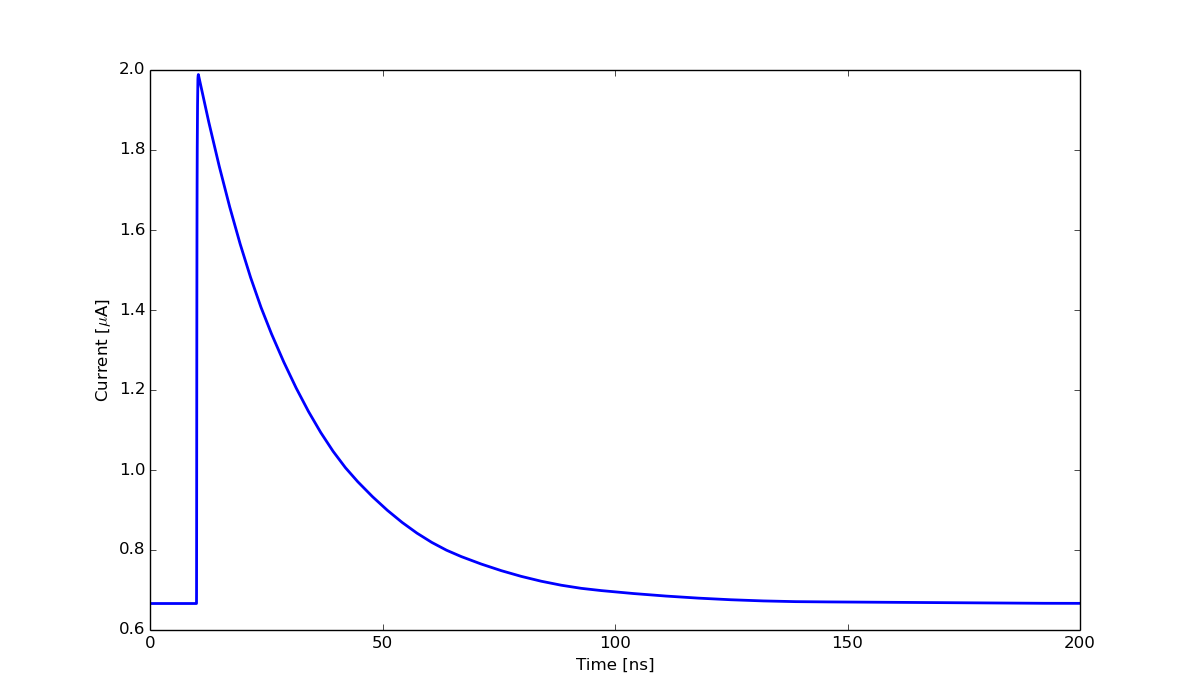
\includegraphics[width=\linewidth]{Graphics/SPAD/SingleCurrentFINAL}
  {\caption*{Fig. 2.4: The current of a simulated SPAD measured through $R_q$. With values of $R_q=500k\Omega, R_d=1k\Omega, C_d=50fF$ and $C_q=20fF$, there is an exponential rise time $\tau_d=0.07ns$ and fall time $\tau_r=35ns$.}}
\end{figure}

The gain is defined to be the number of charge carriers produced per avalanche and one can calculate it by the integral of the current and dividing through by the elementary charge, $q=1.602\times 10^{-19}$. This is typically in the order of $10^5-10^7$ - a gain comparable to PMTs. For a SPAD with a integrated quenching circuit, the gain is generally well-defined due to the uniformity of the internal capacitances: \cite{gundacker2020}

\[
   G=\frac{Q}{e}=\frac{(C_d+C_q)V_{ov}}{e} \tag{2.3}
\]

\noindent One of the properties of a SPAD is that, when a photon is detected, the current remains flowing through its terminals unless the device is quenched. Thus, the SPAD acts as a binary device and its behaviour is independent of the number of photons impinging on the device\footnote{This is why a SPAD is sometimes known as a Geiger-mode avalanche photodiode (GM-APD) in the literature.}; we cannot differentiate between the arrival of single photons and many photons. This issue is resolved in the case of a SiPM by implementing many SPADs in parallel.

\subsection{SiPMs}

\subsubsection{Overview}

SiPMs are formed by connecting many SPADs in parallel; for example, a $1\times 1 mm^2$ SiPM with a $50\mu m$ microcell pitch contains $400$ individual SPADs. Since the SPADs are connected in parallel, they are independent of each other and hence, when multiple photons impinge on the SiPM at the same time, an equivalent number of microcells are fired. Each microcell contributes to the output signal; if $N$ photons are detected by $N$ microcells, the output signal is $N$-times higher than that of a single photon.  Thus, we are able to count the number of photons detected by the device. Fig. 2.5 shows a schematic diagram of a SiPM.

\begin{figure}[h]
  \includegraphics[width=\linewidth]{Graphics/"SiPMDiagram"}
  {\caption*{Fig. 2.5: Taken from \cite{renker2006}. Schematic diagram of a SiPM. To prevent optical and electrical interference, each microcell is separated by a `dead region'. The fill factor of a SiPM refers to the ratio of the active cell area over the total area.}}
\end{figure}

\noindent An equivalent circuit of a SiPM is given in Fig. 2.6. The circuit is similar to the SPAD case but with the addition of a passive element that contains the unfired parallel microcells and a parasitic component due to the grid. \cite{gundacker2020} Using standard circuit rules, it is easy to show that having $N$ microcells in parallel results in resistors and capacitors taking values of $R/N$ and $N\cdot C$ respectively. Fig. 2.6 also takes into account the number of microcells that are fired, $N_f$. Thus, the number of microcells that contribute to the passive component is given by $N-N_f$.

\begin{figure}[h]
\includegraphics[width=\linewidth]{Graphics/"SiPMEquiv"}
  {\caption*{Fig. 2.6: Taken from \cite{gundacker2020}. An equivalent circuit of a SiPM.}}
\end{figure}

\noindent The individual parameters in a SiPM, which need to be known for the model simulation, can be extracted experimentally. The quenching resistor, $R_q$, and the breakdown voltage, $V_{br}$, can be determined from the forward and backward IV (current-voltage) characteristics. Several methods in measuring \(V_{br}\) using the IV curve are compared in \cite{nagai2019}. From Eq. 2.3, we can determine $C_d+C_q$ by measuring the gain. Finally, a CV plotter can be used to measure the conductance, $Y_m$, and the capacitance, $C_m$, at the SiPM terminals. It is then possible to write $Y_m$ and $C_m$ in terms of the parameters and therefore, when the value of $C_d+C_q$ is known, we are able to determine $C_d$, $C_q$ and $C_p$. \cite{corsi2006} The one remaining parameter is $R_d$. For this case, $R_d$ can be assumed to have a value around $\sim 1k\Omega$. Simulations show that changing this value around this range does not affect the output greatly. \cite{acerbi2019}

In the following sections, we briefly review some important properties of SiPMs. These are important to know in order to consider the feasibility of using such devices in the spark chamber trigger system.

\subsubsection{Gain}

Since the microcells are independent, the gain of a SiPM is proportional to the number of fired microcells. Using Eq 2.3:

\[
   G =\sum_i G_i= \sum_i \frac{(C_d+C_q)V_{ov}}{e} \tag{2.4}
\]

\noindent This is only true if the microcells are connected in parallel without any additional impedances. In the SiPM equivalent model, we also have to consider the parasitic capacitances. In addition, the output signal is not proportional to the number of fired microcells if the preamplifier input impedance is not zero. \cite{seifert2010} Hence, the gain is no longer linear with respect to the number of fired microcells.

It is worth, at this point, considering the effect of temperature on the gain. It is important to note that the gain is independent of temperature as long as the overvoltage ($V_{bias}-V_{br}$) remains fixed. However, the breakdown voltage, $V_{br}$, does depend on temperature since the mean free path of the charge carriers decreases with increasing temperature. Thus, a higher electric field is required to start the avalanche process effectively increasing $V_{br}$ and lowering the overvoltage for a fixed bias voltage. \cite{gundacker2020} If the bias voltage is not changed to keep the overvoltage fixed, the gain decreases with increasing temperature.

\subsubsection{Photon Detection Efficiency}

The photon detection efficiency (PDE) is the probability that a photon arriving on the detector surface is detected. It is given by:

\[
  PDE= QE(\lambda) \times \epsilon \times P_{T}(V_{ov},\lambda) \tag{2.5}
\]

\noindent where $QE$ is the quantum efficiency, \(\epsilon\) is the fill factor and \(P_{T}\) is the probability of successfully triggering an avalanche. \(P_{T}\) depends on the overvoltage since the triggering probability depends on the electric field; a higher overvoltage increases \(P_{T}\). The wavelength dependence is due to different absorption depths in the silicon for different wavelengths. The fill factor, $\epsilon$, is the ratio of the active microcell region to the total SiPM area. \cite{acerbi2019}

\begin{figure}[h]
\includegraphics[width=\linewidth]{Graphics/"SiPMPDE"}
  {\caption*{Fig. 2.7: Taken from \cite{sensl2011}. How the PDE is affected by the photon wavelength. A higher overvoltage also increases the PDE since the microcell triggering probability is increased.}}
\end{figure}

\noindent By definition, \(0< QE, \epsilon, P_{T} <1\), so the PDE is maximised when all 3 factors are optimised. QE values as high as 0.98 have been achieved. \cite{firstsensor} Recent advances since 2010 have led to many SiPMs having comparable PDE values up to $60\%$. \cite{gundacker2020} Fig. 2.7 is an example of how the PDE varies with wavelength.

\subsubsection{Primary Noise}

Due to the high bias voltage, it is possible for microcells to be randomly triggered by thermally generated carriers. These dark counts follow a Poisson distribution and forms the primary noise for a SiPM. \cite{cova1996} It follows that reducing the bias voltage reduces the dark count rate (DCR).

The thermal generation of carriers and hence, the DCR obviously depends on the temperature and Fig. 2.8 shows this dependence; at $20^\circ C$, the DCR $\sim 1\times 10^5 \ cps \ mm^2$ where $cps$ is the counts per second. In general, the DCR halves about every $10^\circ C$ and at low temperatures, tunnelling effects dominate dependent on the internal electric field. As seen in Fig. 2.8, the DCR saturation at low temperatures is higher for a SiPM designed with a standard internal field structure than a low field one. \cite{acerbi2017}

\begin{figure}[h]
\includegraphics[width=\linewidth]{Graphics/"DCRTempDependence"}
  {\caption*{Fig. 2.8: Taken from \cite{acerbi2017}. The DCR decreases as the temperature decreases until it reaches a baseline value where tunnelling effects dominate.}}
\end{figure}

\noindent It is interesting to note that there is evidence so suggest that only a small percentage of microcells are responsible for most of the DCR: "some pixels have very high DCR compared to the median DCR value". \cite{mandai2012}

\subsubsection{Correlated Noise}

Noise as a result of primary firing microcells is known as correlated noise (Fig. 2.9). There are two types of correlated noise: i) afterpulsing and ii) optical crosstalk. Afterpulsing is the result of trapped charged carriers during the initial microcell firing process. These trapped carriers are then released after the initial signal to create subsequent signals that are lower in amplitude since the microcell has not fully recovered. Afterpulsing can also be optically induced: each charge carrier in an avalanche produces approximately $3\times 10^5$ secondary photons. \cite{lacaita1993} These secondary photons can be absorbed by the same microcell triggering another avalanche. Afterpulses increase an individual microcell's overall recovery time.

\begin{figure}[h]
\includegraphics[width=\linewidth]{Graphics/"CorrelatedNoise"}
  {\caption*{Fig. 2.9: Taken from \cite{acerbi2019}. Examples of correlated noise.}}
\end{figure}

\noindent Optical crosstalk relates to the firing of neighbouring microcells due to the primary firing microcell. Similar to optically induced afterpulsing, the secondary photons can induce avalanches in neighbouring microcells. Considering just one adjacent microcell, the crosstalk can be near instantaneous resulting in a signal with twice the amplitude (prompt crosstalk) or it can be delayed (delayed crosstalk). Delayed crosstalk events can generally be separated from the primary event due to the longer timescale. We see a secondary signal whose magnitude is the sum of the recovering primary microcell and the fired secondary microcell. Optical crosstalk can be reduced by adding trenches inbetween microcells; trenches increase the `dead region' of the SiPM and hence, affects the fill factor of the overall cell. \cite{gundacker2020}

A simple model to describe the optical crosstalk probability is that, for $N$ avalanches produced simultaneously via optical crosstalk, $P(N) \propto e^{-N}$. \cite{acerbi2019} Defining the crosstalk probability as the number of multi-photon events over the number of single photon events, a naive calculation gives a theoretical upper bound for the optical crosstalk probability:

\begin{align*}
  P(Crosstalk) &= e^{-1}(1+e^{-1}+e^{-2}+\cdots) \\
  &\to \frac{e^{-1}}{1-e^{-1}} \approx 58.2\%
\end{align*}
